\documentclass[12pt]{article}
\usepackage{tabularx}
\usepackage[table]{xcolor}
\usepackage{hyperref}
\usepackage{float}
\usepackage{graphicx}
\usepackage[utf8]{inputenc}
\usepackage[T1]{fontenc}
\usepackage{lmodern}
\usepackage{amsmath, amssymb}
\usepackage{graphicx}
\usepackage{subcaption}
\usepackage[a4paper,margin=1.5cm]{geometry}
\usepackage{placeins}

\title{Integration Project -- Model Predictive Control (MPC)\\[0.3cm]
Modeling and Control of a Transport Network}
\author{Clément Milcent, Kevin Armel Wassa, Mathis Poteau}
\date{January 2025}

\begin{document}

\maketitle

\newpage
\tableofcontents
\newpage

\section{Introduction}

In zone-based evacuation planning, the region to evacuate is divided into zones, and each zone must be assigned a path to safety and departure times along the path. Zone-based evacuations are highly desirable in practice because they allow emergency services to communicate evacuation orders and to control the evacuation more precisely. Zone-based evacuations may also be combined with contraflows (to maximize the network capacities) and may impose additional constraints on the evacuation path (e.g., path convergence) and the departure times (e.g., non-preemption). This project focuses on the modeling and optimal control of a transport network represented as a directed graph.  
The objective is to describe the evolution of the volumes stored in the different components of the network and to formulate a Model Predictive Control (MPC) problem in order to optimize the global behavior of the system over a finite time horizon.

First, a mathematical model of the network dynamics is introduced, together with the associated physical constraints.  
Then, a convex relaxation of the model is proposed in order to make the optimal control problem tractable.  
Finally, a finite-horizon optimal control problem is formulated.

\section{Network Model}
The transport network is represented by a directed graph $G = (V,E)$ composed of two types of nodes:
\begin{itemize}
    \item $\mathcal{T}$: set of \textbf{tanks} ,
    \item $\mathcal{X}$: set of \textbf{transport cells} .
\end{itemize}

The set of vertices is given by $V = \mathcal{T} \cup \mathcal{X}$, with $\mathcal{T} \cap \mathcal{X} = \emptyset$. The evolution of the evacuation network is described in discrete time. Time is discretized with a constant sampling period $h > 0$:
\[
t_k = k h, \quad k = 0,1,\dots,K.
\] 
At each instant, the state of the system is characterized by the number of vehicles stored in each tank $x_T$ and in each cell $x_i$. Control decisions mainly act on the tanks through control variables $u_T$, which regulate the number of vehicles injected into the network. Interactions between the different elements are described by flows \(f_{ij}\), representing the number of vehicles moving from cell $i$ to cell $j$, while the final exits of the network are represented by the variables $\mu_i$ associated with terminal cells. This formulation allows for precise tracking of vehicle propagation throughout the network, accounts for congestion effects, and provides a basis for a model predictive control problem aimed at optimizing evacuation over a finite time horizon under physical and operational constraints.



\subsection{State and control variables}

For each discrete time step $k$, the following variables are defined:
\begin{itemize}
    \item $x_T(k)$: number of cars stored in tank $T \in \mathcal{T}$,
    \item $x_i(k)$: number of cars stored in cell $i \in \mathcal{X}$,
    \item $u_T(k) \in [0,1]$: control associated with tank $T$,
    \item $f_{ij}(k) \ge 0$: flow from node $i$ to node $j$,
    \item $\mu_i(k)$: outflow leaving the network from terminal cells.
\end{itemize}

\subsection{Demand and supply functions}


The dynamics of vehicle flow within each transport cell are described using demand and supply functions. The \textbf{demand function} represents the potential outflow from a cell based on the number of vehicles currently present, the cell’s length, and its velocity, while allowing modulation through a control  : we assume that we can control the speed of the vehicles. In contrast, the \textbf{supply function} models the capacity of a cell to accept incoming vehicles, which decreases as the cell becomes congested. Together, these functions account for congestion effects and flow limitations, ensuring that vehicle movements remain physically realistic and that control actions respect the network's capacity constraints. This formulation is essential for designing an effective model predictive control strategy, as it provides a clear link between the state of the network (vehicle densities) and the possible flows between cells.


\paragraph{Demand function}

The demand function is defined as:
\[
d_i(x_i(k)) = \gamma_i \min\left( \frac{v_i}{l_i} x_i(k),\; C_i \right),
\]
where $v_i$ denotes the velocity, $l_i$ the length of the cell, $C_i$ the maximum capacity, and $\gamma_i \in [0,1]$ is a control parameter used to regulate the flow.

\paragraph{Supply function}

The supply function is given by:
\[
s_i(x_i(k)) = \max\left(c_i - w_i x_i(k),\; 0\right),
\]
where $c_i$ is a capacity constant and $w_i$ is a saturation coefficient.

\subsection{Flow definitions}

The vehicle flows in the network are defined to capture physical limitations and capacity constraints. The \textbf{flow between two cells} is limited by the demand of the upstream cell and the supply of the downstream cell, ensuring realistic traffic propagation. When multiple cells converge into a single cell, the incoming flow is distributed proportionally to the demand of each upstream cell while respecting the capacity of the downstream cell. The \textbf{flow from a tank to a cell} is controlled by the tank’s control variable and is limited by the supply of the target cell. For terminal cells with no successors, the \textbf{outflow from the network} corresponds directly to the demand of the cell. Finally, flows from transport cells back to tanks or upstream cells are prohibited, reflecting the irreversibility of the evacuation. These definitions link the network state and control decisions to the actual flows between cells and tanks, while respecting congestion and capacity constraints.



\paragraph{Cell-to-cell flow}

For two transport cells $i,j \in \mathcal{X}$, the flow is defined as:
\[
f_{ij}(k) = \min\left(d_i(x_i(k)),\; s_j(x_j(k))\right).
\]

\paragraph{Many cells to a single cell flow}
We have $ m \in \mathcal{X}$ cells that all lead to a single cell $j \in \mathcal{X}$. The flow is defined as : 
\[
    \forall i \in [1,m],\ f_{ij} = \min\ (\beta d_i(x_i(k)),s_j(x_j(k)))
\]

\[
    \text{with} \,\beta=\min(\frac{s_j(x_j(k))}{\sum_{i=1}^{m}{d_i(x_i(k))}},1)
\]

\paragraph{Tank-to-cell flow}

For a tank $T \in \mathcal{T}$ and a cell $j \in \mathcal{X}$:
\[
f_{Tj}(k) = \min\left(u_T(k),\; s_j(x_j(k))\right).
\]

\[
    \text{with} \, u_T(k)\ \le \ x_T(k)
\]

\paragraph{Outflow from the network}

If a cell $i$ has no successor, the outflow leaving the network is:
\[
\mu_i(k) = d_i(x_i(k)).
\]

\paragraph{One-way evacuation}

Reverse flows from transport cells back to tanks or upstream cells are forbidden:
\[
f_{jT}(k) = 0, \quad \forall j \in \mathcal{X},\ \forall T \in \mathcal{T}.
\]

\[
f_{ji}(k) = 0, \quad \forall i,j \in \mathcal{X},\ j \ge i.
\]

\subsection{Discrete-time system dynamics}

The discrete-time dynamics of the network describe the evolution of the number of vehicles in tanks and transport cells. Tank number of vehicles decrease according to the outgoing flows to the cells, while cell number of vehicles increase with incoming flows and decrease with outgoing flows and network outflows. This formulation directly links the flows to the network states.


\paragraph{Tank dynamics}

The evolution of the tank number of vehicles is described by:
\[
x_T(k+1) = x_T(k) - h \sum_{j:\,T \to j} f_{Tj}(k).
\]

\paragraph{Cell dynamics}

The dynamics of the transport cells are given by:
\[
x_i(k+1) = x_i(k)
+ h \left(
\sum_{j:\,j \to i} f_{ji}(k)
- \sum_{m:\,i \to m} f_{im}(k)
- \mu_i(k)
\right),
\quad i \in \mathcal{X}.
\]

\subsection{Physical constraints}
The system is subject to the following physical constraints. Vehicle volumes in tanks and cells must be non-negative, and flows between cells cannot be negative, as it is impossible to have a negative number of vehicles moving through the network. The control variable $u_T$, representing the number of vehicles leaving a tank, cannot exceed the volume available in that tank, ensuring that no more vehicles are evacuated than are present. Additionally, when multiple cells converge into a single cell $j$, the total incoming flow cannot exceed the supply of the destination cell, which enforces the network's physical limits.

The system is subject to the following constraints:
\[
\begin{cases}
x_i(k) \ge 0, \quad x_T(k) \ge 0, \\
f_{ij}(k) \ge 0, \\
0 \le u_T(k) \le x_T(k).
\end{cases}
\]

When we get $m \in \mathcal{X}$ cells to a single cell $j \in \mathcal{X}$, we add these constraints : 
\[
    \sum_{i=1}^{m}{f_{ij} \le s_j}
\] 


\section{Open-Loop Analysis of a Simple Network}
\subsection{First Network: Line Graph --- Two Tanks and Six Cells}
\begin{figure}[H]
    \centering
    
\includegraphics[width=0.5\textwidth]{figures/line_graph/graph_2Tanks_6cells.png}
    \caption{Network with two Tanks and six Cells}
    \label{fig:simpleNetworkFig}
\end{figure}

First we modeled a simple line graph network with 6 cells and two tanks plugged respectively on the first and the fourth cell as we can see in figure~\ref{fig:simpleNetworkFig}. Each cell has a 200 meters length and a capacity of 1000 vehicles/h. Each vehicle moves at 70 km/h in the cells. The two tanks are initially filled with 100 vehicles.


\subsection{Second Network: Y-shaped Graph --- Two Tanks and Six Cells}
\begin{figure}[H]
    \centering
    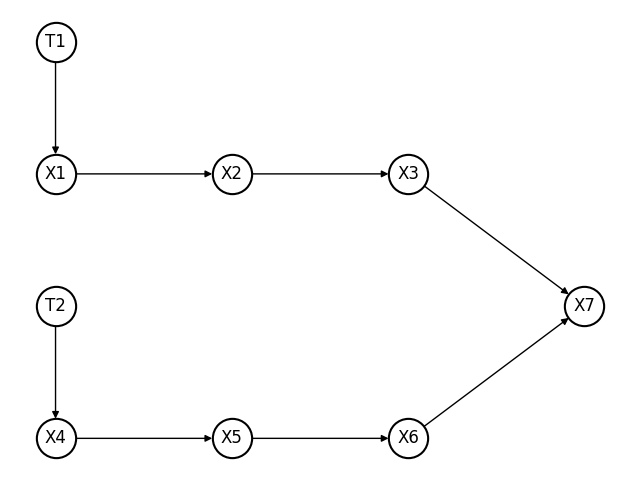
\includegraphics[width=0.5\textwidth]{figures/merge_graph/Graph.png}
    \caption{Network with two Tanks and six Cells}
    \label{fig:complexNetworkFig}
\end{figure}

Then, we modeled a Y-shaped graph network with 7 cells and two tanks plugged respectively on the first and the fourth cell as we can see in figure~\ref{fig:complexNetworkFig}. Each cell has a 200 meters length and a capacity of 1000 vehicles/h. Each vehicle moves at 70 km/h in the cells. The two tanks are initially filled with 100 vehicles.


\subsection{Open-Loop Simulation Setup and Results}
To empty the tanks, two naive open-loop strategies were tested. On one hand, both tanks were emptied simultaneously and, on the other hand, both tanks were fully emptied one after the other, beginning with the second tank. Both strategies were simulated for each of the networks and compared in figure~\ref{fig:simpleNetwork_tankEmptying} and figure~\ref{fig:complexNetwork_tankEmptying}. The control variable $u_T$ was set to the constant value of 100 vehicles so that it did not constrain tanks'outflows. Therefore, these simulations correspond to the best evacuation time for both strategies, in the case of a constant control variable. 

\begin{figure}[h!]
    \centering
    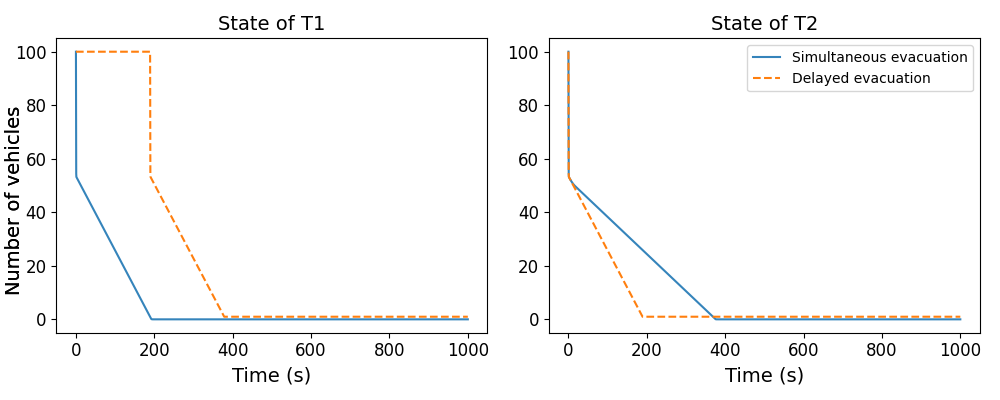
\includegraphics[width=0.7\textwidth]{figures/line_graph/Open_loop/tanks_L200.png}
    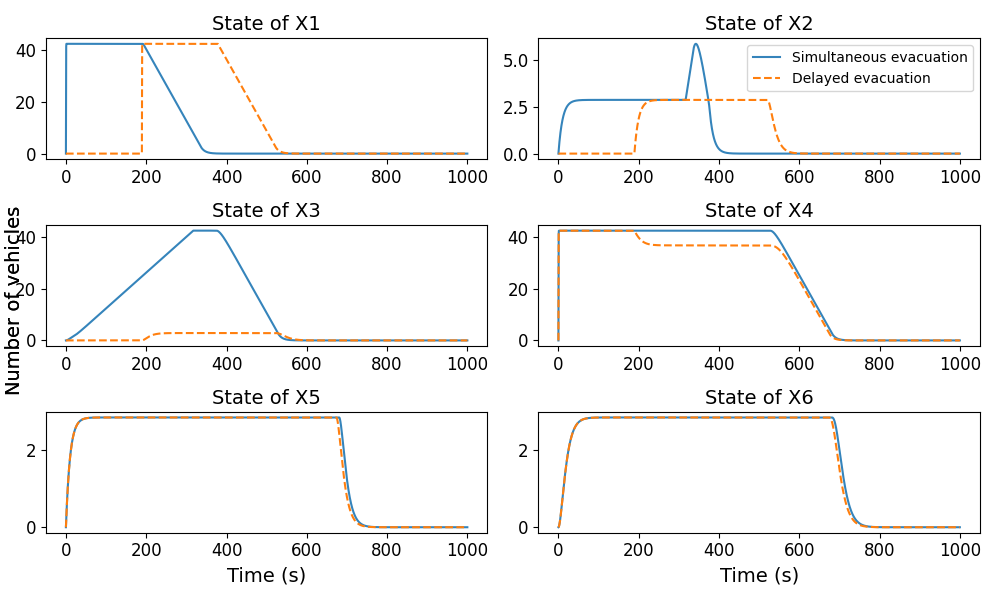
\includegraphics[width=0.7\textwidth]{figures/line_graph/Open_loop/cells_L200.png}
    \caption{Two different evacuation strategies tested for the line graph : simultaneous or delayed evacuation}
    \label{fig:simpleNetwork_tankEmptying}
\end{figure}
\FloatBarrier
 
\begin{figure}[h!]
    \centering
    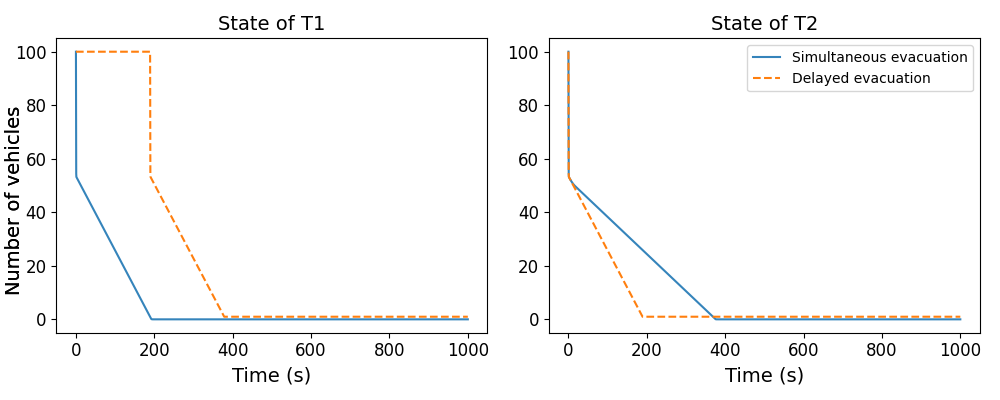
\includegraphics[width=0.7\textwidth]{figures/line_graph/Open_loop/tanks_L200.png}
    \caption{State of the tanks -- Two different evacuation strategies tested for the Y-shaped graph : simultaneous or delayed evacuation}
    \label{fig:complexNetwork_tankEmptying}
\end{figure}
\FloatBarrier

\begin{figure}[h!]
    \centering
    
\includegraphics[width=0.7\textwidth]{figures/merge_graph/Open_loop/cells_L200.png}
    \caption{State of the cells -- Two different evacuation strategies tested for the Y-shaped graph : simultaneous or delayed evacuation}
    \label{fig:complexNetwork_tankEmptying}
\end{figure}
\FloatBarrier

When both tanks are emptied simultaneously in the line graph, there is more stress on cell X4 than for delayed evacuation. This can be explained by the addition of vehicles coming from the first and second tanks, which accumulate at cell 4. In the Y-shaped graph, the same results are observed. There is indeed more stress on cell X7 as this is where both branches merge but also on cells X3 and X6, the closest cells to X7. This is due to the "back-propagation" of saturation on transport cells, i.e. when a cell saturates, the straight upstream cells cannot evacuate their vehicles so they store more of them and end up saturating too. Besides, the saturation limit of each cell is about 42.5 vehicles, corresponding to the maximum number of vehicles that a 200m long road portion can contain (considering average vehicle length of 4.7m).
Note that only one lane is used here for evacuation. 

In the line graph, cells X5 and X6 do not store more than three vehicles. This is due to the absence of tanks or merge downstream so they can evacuate vehicles more easily as cell capacity is not a constraint anymore.

Furthermore, note the symmetry of the Y-shaped graph, causing it to show a symmetric behaviour on both branches in the case of simultaneous evacuation as the control variable is also identical.

Regarding the performance of each strategy, delayed evacuation is slightly quicker than simultaneous one in the line graph configuration, certainly because it reduces saturation. However, it is less suitable to the Y-shaped graph. This can be explained because delayed evacuation does not take advantage of the two parallel branches. 




\section{Model Predictive Control Formulation}
The original flow model relies on $\min(\cdot)$ operators between demand and supply functions. It is these $\min(\cdot)$ operators that introduce nonlinearities and make the constraints non-convex. Such non-convexity prevents the use of efficient optimization methods within a model predictive control framework. 


\subsection{Convex Relaxation of the Flow Model}
To ensure convexity, the $\min(\cdot)$ operators are replaced by inequality constraints, and the flows are treated as independent decision variables $\bar{f}_{ij}$. This relaxation yields a convex optimization problem while preserving the essential physical limitations of the network \cite{ref4}.
\[
0 \le \bar{f}_{ij}(k) \le d_i(x_i(k)),
\]
\[
\sum_{j:\,j \to i} \bar{f}_{ji}(k) \le s_i(x_i(k)).
\]
Relaxing non-convex constraints in MPC involves replacing difficult constraints with convex approximations that are easier to solve. This approach works because the relaxed constraints define a larger feasible set, guaranteeing the existence of a solution and allowing the use of efficient convex solvers.



\subsection{MPC Problem Statement : Finite-horizon optimal control problem}
A prediction horizon of length $K$ is considered, together with the following cost function:
\[
J = \sum_{k=0}^{K} \left( \sum_{i \in \mathcal{X}} x_i(k) + \sum_{T \in \mathcal{T}} x_T(k) \right).
\]

A quadratic cost function is commonly used in MPC formulations to penalize large state deviations and smooth control actions. In the present context, such a cost would strongly penalize high congestion levels and promote more homogeneous traffic distributions. However, unlike a linear cost, a quadratic criterion loses the direct interpretation in terms of total time spent in the network. Moreover, it may bias the controller towards avoiding local peaks rather than maximizing global evacuation efficiency. For these reasons, a linear cost was preferred in this work.

The objective is to minimize $J$ subject to:
\begin{itemize}
    \item control constraints:
    \[
    0 \le u_T(k) \le x_T(k), \quad \gamma_i \in [0,1],
    \]
    \item flow constraints:
    \[
    \sum_{m:\,i \to m} \bar{f}_{im}(k) \le d_i(x_i(k)),
    \]
    \[
    \sum_{j:\,j \to i} \bar{f}_{ji}(k) \le s_i(x_i(k)),
    \]
    \[
    \sum_{j:\,T \to j} f_{Tj}(k) \le u_T(k)\, x_T(k),
    \]
    \item system dynamics,
    \item no reverse flows,
    \item given initial condition $x(0)$.
\end{itemize}
\subsection{Numerical Implementation of the MPC Controller}
The numerical solution to the MPC problem was performed using the cvxpy package, an open source Python-embedded modeling language for convex optimization problems, and the GUROBI solver to increase computational power.

\begin{figure}[H]
    \centering
    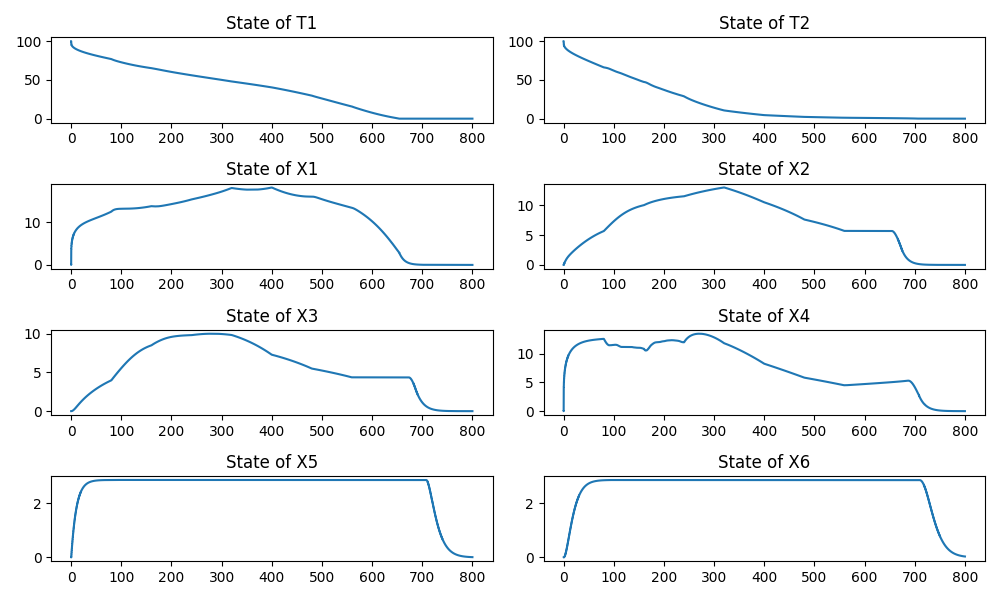
\includegraphics[width=0.7\textwidth]{figures/line_graph/MPC/cells_tanks_8000iter_hor1600.png}
    \caption{MPC solution for the line graph with a horizon of 1600 steps}
    \label{fig:MPC_1600hor}
\end{figure}

The MPC results are displayed on figure \ref{fig:MPC_1600hor}. They don't contain any saturation as the downstream cells from the tanks do not store more than 20 vehicles, although their capacity enable them to store 42,5 of them. The second tank T2 is emptied quicker than the first one T1. The outflow from cells X4, X5 and X6 equals fmax, the maximal flow allowed,  without storing too much vehicles because they store exactly enough vehicles so that fmax is the minimum term in the expression of the demand function.


\section{Coupling the MPC Controller with the Simulator}
\subsection{Simulator Description}
The simulator implements a discrete-time traffic flow model based on the Cell Transmission Model (CTM). The road network is represented as a directed graph composed of tanks and road cells. Each cell is characterized by demand and supply functions, introducing nonlinearities and capacity constraints.

At each time step, traffic flows are computed as the minimum between upstream demand and downstream supply, ensuring conservation of vehicles and congestion effects. The state of each tank and cell is then updated according to mass balance equations.

As we can see in figure ~\ref{fig:CL_MPC_Sim}, when coupled with the MPC controller, the simulator applies the optimal control actions computed by the MPC and propagates the system dynamics forward in time. This closed-loop simulation allows the evaluation of the controller performance on a realistic nonlinear traffic model.

\begin{figure}[H]
    \centering
    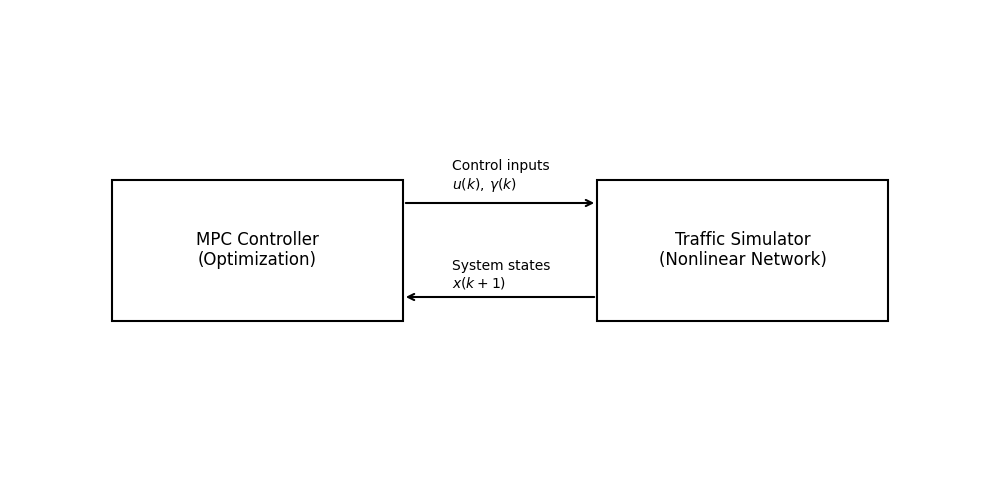
\includegraphics[width=0.7\textwidth]{figures/schemabloc.png}
    \caption{Closed-Loop MPC–Simulator Architecture}
    \label{fig:CL_MPC_Sim}
\end{figure}
\subsection{Closed-Loop Control Architecture}
The control strategy implemented in this work follows a receding horizon
principle based on Model Predictive Control (MPC). At each control iteration,
the optimization problem is formulated and solved over a finite prediction horizon of
length $n_h$. Once the optimization problem is solved, optimal trajectories for both the
control inputs and the system states are obtained over the entire prediction
horizon $n_h$. However, instead of applying the full sequence of optimal
control actions, only the first half of the computed control inputs is
implemented on the simulator. More precisely, assuming that the horizon length
$n_h$ is divisible by two, only the first $\frac{n_h}{2}$ control steps are applied,
while the remaining ones are discarded. For instance, if the prediction
horizon is chosen as $n_h = 20$, the controller applies the optimal inputs over
the next $10$ time steps.

After these $\frac{n_h}{2}$ control actions have been applied, the simulator propagates
the nonlinear dynamics of the traffic network and provides updated state
measurements. These new states are then used to reinitialize the MPC problem,
and a new optimization is solved over a shifted horizon. This procedure is
repeated iteratively until the final simulation time is reached. Such a
receding horizon strategy improves robustness with respect to modeling
uncertainties and disturbances, while maintaining a reasonable trade-off
between computational complexity and control performance.

\subsection{Closed-Loop Simulation Results}
This part is fed with both the  MPC results and the simulator outputs based on the MPC solution.\\ Both results are displayed on the same plots so that they can be compared.
The MPC is run over a finite horizon of 200 for 2000 iterations.

\subsubsection{Line graph}


\begin{figure}[h!]
    \centering
    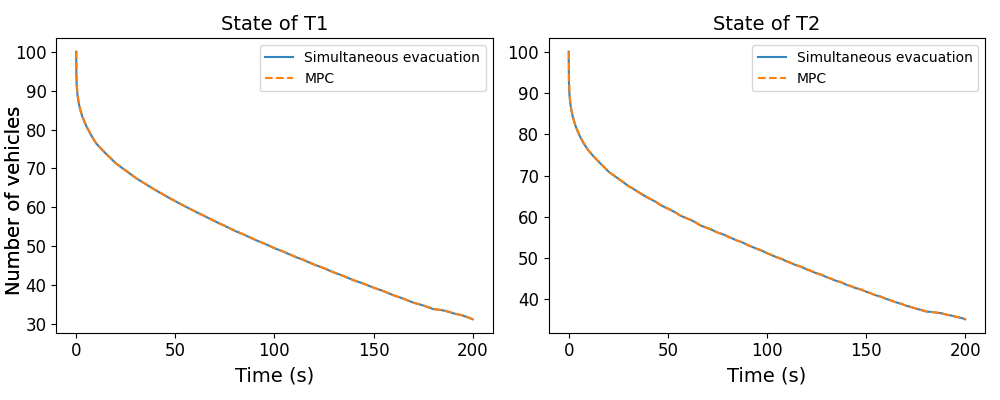
\includegraphics[width=0.6\linewidth]{figures/line_graph/Simulator_Mpc_coupled/tank_L200.png}
    \caption{Line graph : MPC tank states}
    \label{fig:MPC_tank_states}
\end{figure}
\FloatBarrier

\begin{figure}[h!]
    \centering
    
\includegraphics[width=0.6\linewidth]{figures/line_graph/Simulator_Mpc_coupled/cells_L200.png}
    \caption{Line graph : MPC cells states}
    \label{fig:MPC_cells_states}
\end{figure}
\FloatBarrier

The simulator matches accurately the MPC plots using MPC solution. Especially the plots of the tanks and the cells $x_1,\ x_4,\ x_5$ and $x_6$. Regarding the other cells, the match is not perfect but the results are still really close. 

\subsubsection{Y-shaped graph}

\begin{figure}[h!]
    \centering
    
\includegraphics[width=0.6\linewidth]{figures/merge_graph/Simulator_Mpc_coupled/tanks_L200.png}
    \caption{Y-shaped graph : MPC tank states}
    \label{fig:MPC_tank_states_many_cells}
\end{figure}
\FloatBarrier

\begin{figure}[h!]
    \centering
    
\includegraphics[width=0.6\linewidth]{figures/merge_graph/Simulator_Mpc_coupled/cells_L200.png}
    \caption{Y-shaped graph : MPC cells states}
    \label{fig:MPC_cells_states_many_cells}
\end{figure}
\FloatBarrier

In the Y-shaped graph configuration, the results are slightly worse than for the line graph. Indeed, larger discrepancies can be observed between the MPC results and those of the simulator. However, the general trends are still respected, which indicates that the MPC is able to capture the main dynamics of the system despite the observed deviations.

To conclude, these results show that the previously performed convex relaxations do not distort the model dynamics. Therefore, the MPC solution can be found by controlling the vehicles' speed.

\section{Results and Performance Analysis}
\subsection{Comparison Between Open-Loop and Closed-Loop Behavior}

Table~\ref{tab:tableComparisonOL_MPC} compares the time performance of different control strategies. The results show that Model Predictive Control (MPC) with a prediction horizon of 800 and the optimization-based approach lead to very similar outcomes, with times of 733 s and 732 s respectively, indicating nearly identical closed-loop behavior. In contrast, open-loop strategies result in significantly longer times. When the two tanks empty sequentially, the time increases to 902 s, while it reaches 836 s when both tanks empty simultaneously. These results clearly highlight the advantage of closed-loop control strategies, which provide a more efficient dynamic management of the system and significantly reduce the time required to reach the condition where only one vehicle remains in zone X6.
\begin{table}[H]
    \centering
    \begin{tabularx}{\textwidth}{|X|c|c|}
        \hline
        \rowcolor{gray!20}
        Used Method & Evacuation time (in seconds) & Cost \\ \hline
        MPC with horizon 1600 & 744 & 762723 \\ \hline
        Open-loop delayed evacuation & 737 & 766 829 \\ \hline
        Open-loop simultaneous evacuation & 744 & 761588 \\ \hline
        Open-loop simultaneous evacuation & 744 & 761588 \\ \hline
    \end{tabularx}
    \caption{Comparison Between Open-Loop and Closed-Loop Behavior}
    \label{tab:tableComparisonOL_MPC}
\end{table}

\subsection{Impact of MPC on Congestion Reduction}

In order to intentionally create a congestion phenomenon in the line graph,
the parameters of one $X_5$ were modified. Its speed was reduced to $35\,\mathrm{km/h}$ and its maximum flow capacity was limited to $200$ vehicles per hour, while all other cells retained
their nominal parameters. In addition, the length of each road segment was set
to $200m$.

These parameter changes directly affect both the demand and supply functions
of cell $X_5$. The reduction in speed lowers the demand function, while the
decrease in maximum flow introduces a strict capacity constraint. As a result,
cell $X_5$ becomes a limiting element in the traffic network, causing vehicles
to accumulate upstream as we can see in figure~\ref{fig:OL_cells_cong}. This configuration deliberately reproduces a
congestion scenario, allowing the behavior of the network to be analyzed under
bottleneck conditions.

\begin{figure}[H]
    \centering

    \begin{subfigure}[b]{0.45\linewidth}
        \centering
        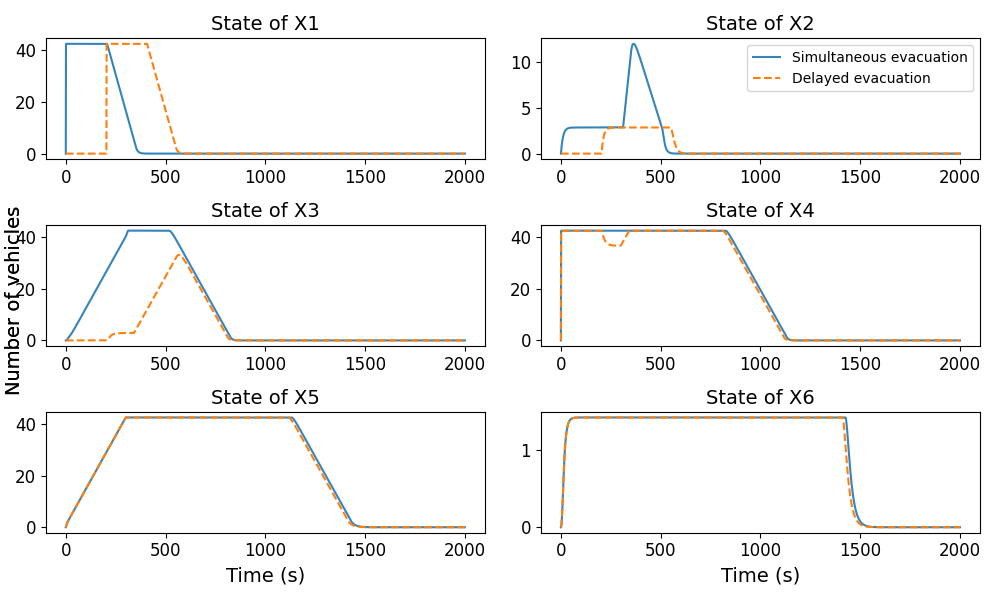
\includegraphics[width=\linewidth]{figures/line_graph/Congestion/cells_OL.png}
        \caption{Open-loop behavior}
        \label{fig:OL_cells_cong}
    \end{subfigure}
    \hfill
    \begin{subfigure}[b]{0.45\linewidth}
        \centering
        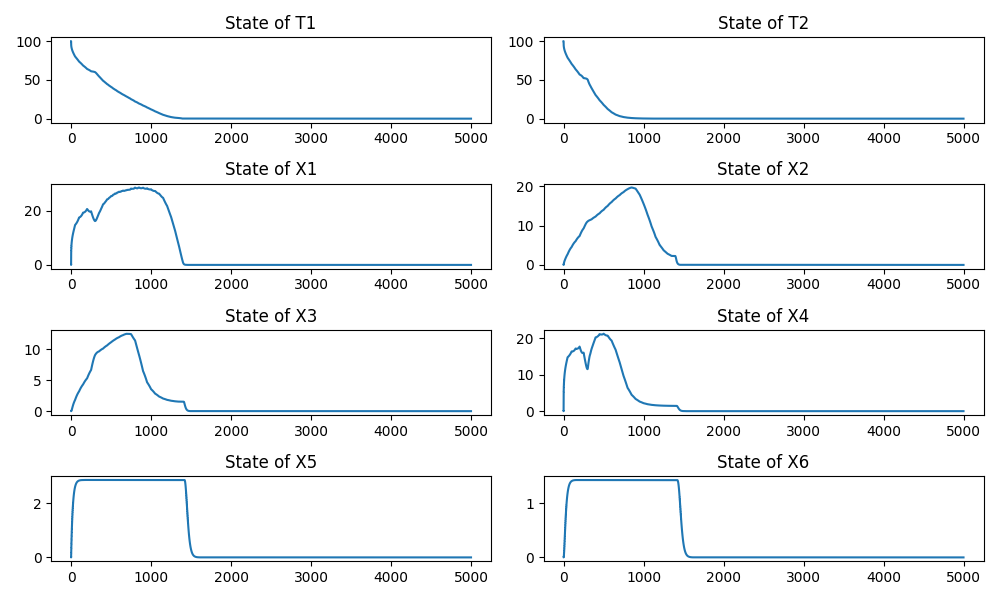
\includegraphics[width=\linewidth]{figures/line_graph/Congestion/tanks_cells_50000iter.png}
        \caption{Closed-loop MPC behavior}
        \label{fig:CL_cells_cong}
    \end{subfigure}

    \caption{Cell states under congestion conditions for the line network}
    \label{fig:cells_congestion_comparison}
\end{figure}
In the open-loop case, severe congestion is observed, as several upstream cells
($X_5$, $X_4$, $X_3$, and even $X_1$) reach approximately $42$ vehicles, which
corresponds to the maximum occupancy of a cell. This indicates an uncontrolled
propagation of congestion caused by the bottleneck at cell $X_5$.

In contrast, in the closed-loop MPC case with a horizon of $1000$, none of the cells reaches this maximum
capacity. Although some vehicle accumulation remains due to the reduced
capacity of $X_5$, the MPC controller effectively regulates upstream inflows,
keeping vehicle densities bounded and preventing full congestion. Moreover, the
evacuation times remain comparable in both cases, showing that congestion
mitigation is achieved without significantly impacting overall throughput.


\section{Conclusion and Perspectives}

This study focused on the application of MPC to a Cell Transmission Model, made possible by convex relaxations. The performance of the control algorithm was compared to naive evacuation strategies. Although the evacuation time obtained by the MPC does not indicate that it improves evacuation performance compared to these simple strategies, several objections can be raised. Firstly, it is important to note that the result calculated by the MPC is already very good, as it is very close to the maximum flow value allowed in the model, which cannot be exceeded. Secondly, the MPC calculates a strategy that does not saturate the network, unlike the other two methods, which produce poorer performance when the control applied does not allow them to saturate. Furthermore, the current simulator model does not seem to penalise congested traffic. Finally, the MPC solution depends on the cost function selected. There may be a cost function that slightly improves the evacuation time obtained, such as introducing a term that rewards vehicle exit, for example.


\begin{thebibliography}{9}

\bibitem{ref1}
Mohd. Hafiz Hasan and Pascal Van Hentenryck,
Large-scale zone-based evacuation planning—Part I: Models and algorithms,
Special Issue on Celebrating 50 Years of Networks: Part 1,
Volume77, Issue1, Pages 127-145.

\bibitem{ref2}
Christian Rosdahl, Gustav Nilsson and Giacomo Como,
On Distributed Optimal Control of Traffic Flows in Transportation Networks,
Department of Automatic Control, Lund University,
Lagrange Department of Mathematical Sciences, Politecnico di Torino.

\bibitem{ref3}
Christian Rosdahl,
MSc Thesis : Distributed Control of Dynamic Flows in Traffic Networks,
Department of Automatic Control, Lund University.

\bibitem{ref4}
R.M Lewis and R.B Vinter,
Relaxation of optimal control problems to equivalent convex programs,
Journal of Mathematical Analysis and Applications,
Volume 74, Issue 2, April 1980, Pages 475-493.


\end{thebibliography}

\newpage
\listoffigures



\end{document}
